\documentclass[tikz,border=10pt]{standalone}
\usepackage{tikz}
\usetikzlibrary{positioning,shapes.geometric,arrows.meta,calc}
\usepackage{amsmath}

\begin{document}
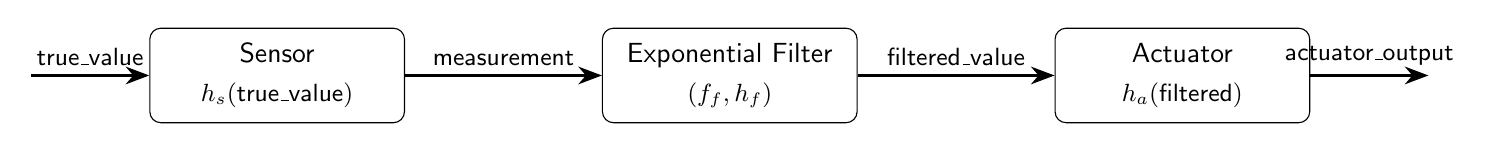
\begin{tikzpicture}[
    node distance=2.5cm,
    block/.style={rectangle, draw, fill=white, text width=3cm, text centered, rounded corners, minimum height=1.2cm, font=\sffamily},
    arrow/.style={-{Stealth[length=3mm]}, thick},
    signal/.style={font=\small\sffamily}
]

% Blocks
\node[block] (sensor) {Sensor\\[2pt]{\small $h_s(\text{true\_value})$}};
\node[block, right=of sensor] (filter) {Exponential Filter\\[2pt]{\small $(f_f, h_f)$}};
\node[block, right=of filter] (actuator) {Actuator\\[2pt]{\small $h_a(\text{filtered})$}};

% Input signal
\coordinate[left=1.5cm of sensor] (input);

% Output signal
\coordinate[right=1.5cm of actuator] (output);

% Arrows with labels
\draw[arrow] (input) -- node[above, signal] {true\_value} (sensor);
\draw[arrow] (sensor) -- node[above, signal] {measurement} (filter);
\draw[arrow] (filter) -- node[above, signal] {filtered\_value} (actuator);
\draw[arrow] (actuator) -- node[above, signal] {actuator\_output} (output);

\end{tikzpicture}
\end{document}
